\chapter{Equivalência e Ordem}\label{cap:EqOrder}

\epigraph{``O problema do mundo hoje é que as pessoas inteligentes estão cheias de dúvidas, e as pessoas idiotas estão cheias de certezas...''}{Bertrand Russell}

\section{Introdução}\label{sec:IntroEqOrder}

No Capítulo \ref{cap:Relations} anterior este documento apresentou ao leitor a ideia de relações sobre conjuntos, em especial foram tratadas as relações binários sobre um conjunto dado. Agora nesta seção será apresentada de forma profunda duas classes relações binárias muito importantes, sendo elas as relações de equivalência e de ordem. Como dito em \cite{abe1991-TC, carmo2013}, as relações de equivalência ao lado das relações de ordem são de importância central para toda a matemática, além disso, as relações de equivalência também desempenho importantes papéis nas área de mineração de dados \cite{lin1999data, lingras1998data}, aprendizado de máquina \cite{bar2003learning} e processamento de sinais \cite{li2007equivalent} e imagens \cite{acharya2003classification, myasnikov2018description}. E por sua vez, as relações de ordem também aparecem em diversas áreas de caráter prática tais como processamento de imagens \cite{farias2016image, cressie1998image}, criptografia \cite{giri2008crypto}, otimização \cite{karaman2018partial} e etc.

\section{Relações de Equivalência e Espaço Quociente}\label{sec:Equivalence}

E interessante começar pela pergunta básica, o que seria uma relação de equivalência? Bem, uma resposta satisfatória para essa pergunta é que uma relação de equivalência pode ser entendida como sendo uma forma de parear os elementos de um conjunto que apresentam similaridade entre si com respeito a uma ou mais propriedades específicas, isto é, uma relação de equivalência junta os elementos em pares pela similaridade, definida por algum critério. A seguir será apresentado de forma precisa o conceito de relação de equivalência.

\begin{definicao}[Relação de Equivalência]\label{def:RelacaoEquivalencia}
	Seja $A$ um conjunto uma relação binária $\equiv$ sobre $A$ é dita ser uma relação de equivalência sempre que $\equiv$ for reflexiva, simétrica e transitiva.
\end{definicao}

Além da notação $\equiv$ outros símbolos também são comumente encontrados na literatura para representar relações de equivalência, entre, tais símbolos destacam-se $\approx$ e $\sim$.

\begin{exemplo}\label{exe:Equivalencia1}
	Dado um conjunto $C$ qualquer, a relação de igualdade $(=)$ definida em $C$ é obviamente uma relação de equivalência.
\end{exemplo}

\begin{exemplo}\label{exe:Equivalencia2}
	Dado o conjunto $A =\{a, b, c, d\}$ a relação $R$ definida por $a \mathrel{R} a$, $a \mathrel{R} b$, $b \mathrel{R} a$, $b \mathrel{R} b$, $c \mathrel{R} c$ e $d \mathrel{R} d$, é claramente uma relação de equivalência.
\end{exemplo}

Os Exemplos \ref{exe:Equivalencia1} e \ref{exe:Equivalencia2} permite o leitor perceber uma importante verdade matemática, tal verdade como expressa em \cite{carmo2013} pode ser escrita como: ``objetos iguais são equivalentes, mas objetos equivalentes nem sempre são iguais''.

\begin{exemplo}
	Dado um plano $P$ a relação de paralelismo definido sobre o conjunto de retas de $P$ é uma relação de equivalência, outro exemplo clássico da geometria é a semelhança entre triângulos neste mesmo plano $P$.
\end{exemplo}

\begin{exemplo}
	A relação $R = \{(x, y) \in \mathbb{Z}^2 \mid x \mod 5 = y \mod 5\}$ é uma relação de equivalência\footnote{A expressão $a\mod 5$ com $a \in \{x, y\}$ diz respeito ao resto da divisão inteira de $a$ por 5.}.
\end{exemplo}

\begin{exemplo}
	A relação $I =  \{(x, y) \in PERS^2 \mid x, y \text{ possuem a mesma idade}\}$ é uma relação de equivalência sobre o conjunto de todas as pessoas $(PERS)$.
\end{exemplo}

\begin{exemplo}
	Dado o conjunto de todos os times de futebol do Brasil a relação $T$ definida como $x \mathrel{T} y \Longleftrightarrow x, y \text{ nunca foram rebaixados para a segunda divisão}$, é uma relação de equivalência.
\end{exemplo}

A partir da noção de relação de equivalência é possível como destacado em \cite{abe1991-TC} definir a noção de classes de equivalência.

\begin{definicao}[Classes de Equivalência]\label{def:ClasseEquivalencia}
	Seja $\equiv$ uma relação de equivalência sobre um conjunto $A$, para todo $x \in A$ é definida a classe de equivalência de $x$, denotado por $[x]$, como sendo o conjunto de todos os elementos equivalentes a $x$, simbolicamente tem-se que:
	$$[x] = \{y \in A \mid y \equiv x\}$$
\end{definicao}

Obviamente toda classe de equivalência $[x]$ é um subconjunto do conjunto base. Além disso,  obviamente tem-se que $[x] = \emptyset$ se, e somente se, o conjunto base for vazio.

\begin{exemplo}\label{exe:ClasseEquivalencia1}
	Seja $A = \{0, 1, 2, 3\}$ e $0 \equiv 0$, $1 \equiv 1$, $2 \equiv 2$, $3 \equiv 3$, $0 \equiv 2$, $1 \equiv 3$, $2 \equiv 0$, $3 \equiv 1$ tem-se que: $[0] = \{0, 2\}$, $[1] = \{1, 3\}$, $[2] = \{0, 2\}$ e $[3] = \{1, 3\}$.
\end{exemplo}

\begin{exemplo}
	A relação $a \equiv a$, $b \equiv b$, $c \equiv c$, $a \equiv b$, $b \equiv a$ definida sobre o conjunto $\{a, b, c\}$ é uma relação de equivalência e existem as seguintes classes de equivalência $[a] = [b] = \{a, b\}$ e $[c] =\{c\}$.
\end{exemplo}

\begin{teorema}\label{teo:EquivalenciaPropriedade1}
	Seja $\equiv$ uma relação de equivalência sobre um conjunto $A$ não vazio e sejam $a, b \in A$, tem-se que $a \equiv b$ se, e somente se, $[a] = [b]$.
\end{teorema}

\begin{prova}
	$(\Rightarrow)$ Suponha que $a \equiv b$, assim dado  qualquer $x \in [a]$ tem-se que $x \equiv a$, agora pela transitiva de $\equiv$ é claro que $x \equiv b$ e, portanto, $x \in [b]$, logo $[a] \subseteq [b]$ e com raciocínio similar pode-se concluir que $[b] \subseteq [a]$ e assim pela Definição \ref{def:IgualdadeConjuntos} tem-se que $[a] = [b]$. $(\Leftarrow)$ Suponha que $[a] = [b]$, por $\equiv$ ser reflexiva é claro que $a \equiv a$ e assim $a \in [a]$, mas como $[a] = [b]$ tem-se que $a \in [b]$, e portanto, por definição $a \equiv b$.
\end{prova}

\begin{teorema}\label{teo:EquivalenciaPropriedade2}
	Seja $\equiv$ uma relação de equivalência sobre um conjunto $A$ não vazio e sejam $a, b \in A$, tem-se que $a \not\equiv b$ se, e somente se, $[a] \cap [b] = \emptyset$.
\end{teorema}

\begin{prova}
	$(\Rightarrow)$ Suponha por absurdo que $a \not\equiv b$ e $[a] \cap [b] \neq \emptyset$, logo existe um $x \in A$ tal que $x \in [a] \cap [b]$, mas assim pela Definição \ref{def:IntersecaoConjuntos} tem-se que $x \in [a]$ e $x \in [b]$, logo $x \equiv a$ e $y \equiv b$, mas uma vez que $\equiv$ é simétrica tem-se que $a \equiv x$, e como $\equiv$ é transitiva tem-se que $a \equiv b$, o que contradiz a hipótese, caraterizando um absurdo, consequentemente, se $a \not\equiv b$ tem-se então que $[a] \cap [b] = \emptyset$. $(\Leftarrow)$ Suponha que $[a] \cap [b] = \emptyset$, como $a \in [a]$ e pela hipótese $a \notin [a] \cap [b]$ tem-se que $a \notin [b]$ e, portanto, $a \not\equiv b$.
\end{prova}


\begin{definicao}[Espaço Quociente]\label{def:EspacoQuociente}
	Seja $A$ um conjunto e $\equiv$ uma relação de equivalência sobre $A$, o espaço quociente de $A$ com respeito (ou módulo) $\equiv$, denotado por $A_{/_\equiv}$, é o conjunto de todas as classes de equivalência do conjunto $A$, na linguagem na teoria dos conjuntos tem-se que:
	$$A_{/_\equiv} = \{[x] \mid x \in A\}$$
\end{definicao}

\begin{exemplo}
	Seja $A = \{a, b, c\}$ e $R = \{(a, a), (b, b), (c, c), (a, b), (b, a)\}$ claramente $R$ é uma relação de equivalência e além disso $[a] = [b] = \{a, b\}$ e $[c] = \{c\}$ assim $A_{/_R} = \{[a], [c]\}$.
\end{exemplo}

\begin{exemplo}
	Dado que a relação 
  $$P = \{(x,y) \in \mathbb{Z}_+ \mid x, y\text{ tem o mesmo resto da divisão por } 2\}$$ 
  é uma relação de equivalência sobre $\mathbb{Z}_+$ (a prova fica como exercício ao leitor) tem-se claramente que, 
	$$[0] = \{0, 2, 4, 6, 8, \cdots\}$$
	e
	$$[1] = \{1, 3, 5, 7, 9, \cdots\}$$
	ou seja, $[0]$ é o conjunto dos pares positivos e $[1]$ é o conjunto dos impares positivos, assim claramente tem-se que $\mathbb{Z}_{+/_P} = \{[0], [1]\}$.
\end{exemplo}

Uma fato importante sobre o espaço quociente de uma relação de equivalência $\equiv$ é que sempre que o conjunto base $A \neq \emptyset$ tem-se que $A_{/_\equiv} \neq \emptyset$, e mais do que isso, como mostrado a seguir o espaço quociente é sempre uma partição sobre o conjunto base $A$.

\begin{teorema}
	Seja $\equiv$ uma relação de equivalência sobre um conjunto não vazio $A$, então $A_{/_\equiv}$ é uma partição de $A$.
\end{teorema}

\begin{prova}
	Primeiramente note que como $\equiv$ é uma relação reflexiva tem-se para todo $x \in A$ que $x \in [x]$ e assim claramente $[x] \in A_{/_\equiv}$ e $[x] \neq \emptyset$, satisfazendo assim a condição (1) da Definição \ref{def:ParticaoConjuntos}. Por outro lado, os Teoremas \ref{teo:EquivalenciaPropriedade1} e \ref{teo:EquivalenciaPropriedade2} mostram que dado $[x], [y] \in A_{/_\equiv}$ sempre que $[x] \neq [y]$ tem-se que  $[x] \cap [y] = \emptyset$ e, portanto, a condição (2) da Definição \ref{def:ParticaoConjuntos} é satisfeita, desde que as condições (1) e (2) são satisfeita pelo elementos de $A_{/_\equiv}$ tem-se que $A_{/_\equiv}$ é uma partição de $A$.
\end{prova}

\section{Relações de Ordem}\label{sec:Order}

Em algumas situações é interessante que seja possível definir uma hierarquia entre os elementos de um determinado conjunto, de fato, como dito em \cite{abe1991-TC} diversos campos das ciências empíricas, tais como a área da biologia comparada, são dependentes de construções hierárquicas. Dentro da própria ciência da computação diversas áreas (estrutura de dados, classificação de dado e etc.) também utilizam de ordens de hierarquia. Assim é conveniente apresentar o estudo das relações de ordem e das estruturas existentes envolta de tais relações, para isso apresenta-se primeiro as ideias de pré-ordem e ordem estrita.

\begin{definicao}[Ordem Estrita]\label{def:OrdemParcialEstrita}
	Seja $A$ um conjunto, uma relação $\sqsubset$ sobre $A$, é dita ser uma relação de ordem parcial estrita, ou simplesmente ordem estrita, sempre que $\sqsubset$ for irreflexiva e transitiva.
\end{definicao}

\begin{exemplo}
	A relação $\{(x, y) \in \mathbb{N}^2 \mid (\exists k \in \mathbb{N})[k \geq 1 \land y = x + k	]\}$ é uma ordem estrita.
\end{exemplo}

\begin{exemplo}
	Dado um conjunto $A$ qualquer a relação de ser subconjunto próprio $(\subset)$ é um ordem estrita sobre o conjunto $\wp(A)$.
\end{exemplo}

\begin{exemplo}
	Dado o conjunto $\{1, 2, 3\}$ a relação $\{(1, 2), (2, 3), (2, 2), (1, 3)\}$ não é uma ordem estrita pois $(2, 2)$ é um par pertencente a relação.
\end{exemplo}

\begin{definicao}[Pré-ordem]\label{def:PreOrdem}
	Seja $A$ um conjunto, uma relação $\sqsubseteq$ sobre $A$, é dita ser uma relação de pré-ordem sempre que $\sqsubseteq$ for reflexiva e transitiva.
\end{definicao}

\begin{exemplo}
	Dado o conjunto $\{a, b, c\}$ a relação $\{(a, a), (b, b), (c, c), (b, c), (c, a),$ $(b, a)\}$ é uma relação de pré-ordem.
\end{exemplo}

\begin{exemplo}
	A relação $\{(x, y) \in \mathbb{N}^2 \mid (\exists k \in \mathbb{N})[y = xk]\}$ é uma pré-ordem.
\end{exemplo}

\begin{exemplo}
	A relação $\{(x, y) \in \mathbb{N}^2 \mid x + y \neq x \text{ e } x + y \neq y\}$ não é uma pré-ordem pois não é reflexiva, basta notar que $(0,0)$ não pertence a tal relação.
\end{exemplo}

Aumentando as restrições sobre uma pré-ordem, isto é, adicionando mais propriedades a serem exigidas, é construída a noção de ordem parcial, tal conceito é formalizado a seguir. 

\begin{definicao}[Ordem Parcial]\label{def:OrdemParcial}
	Seja $A$ um conjunto, uma relação $\sqsubseteq$ sobre $A$, é dita ser uma relação de ordem parcial sempre que $\sqsubseteq$ for reflexiva, antissimétrica e transitiva.
\end{definicao}

Como dito em \cite{abe1991-TC} se $\sqsubseteq$ é uma ordem parcial sobre um conjunto $A$, então tem-se que $\sqsubseteq$ organizar (ou ordena) o conjunto $A$ em uma determinada hierarquia (ou ordem), obviamente um mesmo conjunto pode apresentar diferentes ordenações, ou seja, podem existir diversas ordens parciais sobre $A$.

\begin{atencao}
  De forma geral quando $x \sqsubseteq y$ pode ser interpretado como $x$ é anterior ou igual a $y$, entretanto, para o caso especifico das relações de ordem parcial $\leq$ e $\subseteq$ suas semânticas sãos as aquelas que o leitor já conhece, isto é, $x \leq y$ significa $x$ é menor ou igual a $y$ e $X \subseteq Y$ significa que $X$ é subconjunto de $Y$.
\end{atencao}

Além das duas famosas ordens parciais mencionadas acima, a seguir serão apresentados mais algumas ordens parciais.

\begin{exemplo}\label{exe:OrdemParcialSimples}
	As seguintes relações são exemplos de ordens parciais:
	\begin{itemize}
		\item[(a)] $\{(x, y) \in \mathbb{N}^2 \mid (\exists k \in \mathbb{N})[y = x + k]\}$.
		\item[(b)] $\{(x, y) \in \mathbb{N}^2 \mid (\exists k \in \mathbb{N})[y = xk]\}$.
		\item[(c)] Dado um conjunto $A$ de todas as pessoas da terra a relação $x \mathrel{R} y$ se, e somente se, $x$ tem a mesma altura ou é mais alto que $y$, é uma ordem parcial sobre $A$.
	\end{itemize}
\end{exemplo}

Fique atento e note que a ordem no item $(b)$ do Exemplo \ref{exe:OrdemParcialSimples} foi anteriormente usado como exemplo de uma pré-ordem, isso ocorre por que toda ordem parcial é uma pré-ordem.

\begin{exemplo}
	Seja $A = \{a, b, c, d\}$ um conjunto a relação $R$ definida como sendo 
  $$\{(a, a), (b, b), (c, c), (d, d), (a, b), (b, c), (a, c), (a, d)\}$$ 
  é uma ordem parcial sobre $A$.
\end{exemplo}

\begin{exemplo}
	Dado $\{0,1\}$ e a relação $\{(0,0), (0, 1), (1, 1)\}$ é uma ordem parcial.
\end{exemplo}

\begin{exemplo}
	Dado um conjunto $\{0, 1, 2, 3\}$ a relação $\{(0, 0), (0, 1), (2, 2), (1, 2),$ $(0, 2), (3, 3)\}$ não é uma ordem parcial pois o par $(1, 1)$ não pertence a relação e por definição uma ordem parcial deve ser reflexiva.
\end{exemplo}

A partir da ideia de ordem parcial é possível definir o conceito de comparabilidade como se segue.

\begin{definicao}[Comparabilidade]\label{def:Comparabilidade}
	Seja $A$ um conjunto não vazio, $\sqsubseteq$ uma ordem parcial sobre $A$ e seja $x, y \in A$, é dito que $x$ e $y$ são comparáveis sempre que $x \sqsubseteq y$ ou $y \sqsubseteq x$.
\end{definicao}

Como dito em \cite{abe1991-TC, carmo2013} tem-se que a noção de comparabilidade está ligada a ordem em questão, assim pode haver um conjunto $A$ e uma ordem parcial $\sqsubseteq_1$ tal que dois elementos $x$ e $y$ são comparáveis, entretanto, pode haver outra ordem parcial $\sqsubseteq_2$ sobre o mesmo conjunto tal que os elementos $x$ e $y$ não pode ser comparáveis\sidefootnote{Em algumas obras é usado a escrita $x \not\sqsubseteq y$ para esboçar que $x$ e $y$ são incomparáveis por uma ordem parcial $\sqsubseteq$.}.

\begin{exemplo}
	Considere o conjunto $A = \{1, 2, 3\}$ tem-se que $\subseteq$ será obviamente uma ordem parcial sobre $\wp(A)$, agora note que $\{1, 2\} \subseteq A$, portanto, $\{1, 2\}$ e $A$ são comparáveis, por outro lado, $\{1, 2\} \not\subseteq \{1, 3\}$ e $\{1, 3\} \not\subseteq \{1, 2\}$, logo $\{1, 2\}$ e $\{1, 3\}$ são incomparáveis.
\end{exemplo}

\begin{exemplo}
  Dado o conjunto $\mathbb{R}$ e a ordem parcial $\leq$ sobre $\mathbb{R}$ tem-se que todo par de números reais $(x, y)$ é sempre comparável.
\end{exemplo}

Por fim é apresentado a ideia de ordem parcial, pela definição a seguir é fácil para o leitor perceber que toda ordem total é uma ordem parcial, porém, o oposto não é verdade.

\begin{definicao}[Ordem total]
	Uma ordem parcial $\sqsubseteq$ sobre um conjunto $A$ é dita ser total quando para todo par de elementos $x, y \in A$ é comparável.
\end{definicao}

\begin{exemplo}
	São exemplos de ordem totais:
	\begin{itemize}
		\item[(a)] A ordem usual ``menor igual'' $(\leq)$ sobre o conjunto $\mathbb{R}$.
		\item[(b)] A relação $\{(a_0, a_0), (a_0, a_1), (a_0, a_2), (a_1, a_1), (a_1, a_2), (a_2, a_2)\}$ sobre o conjunto $\{a_0, a_1, a_2\}$.
	\end{itemize}
\end{exemplo}

Nesta seção ao apresentar a ideia de relações de ordem isso era feito pelo estudo da relação em si ficando seu conjunto base em segundo plano e com pouco interesse, agora serão considerados simultaneamente os dois conceitos juntos, ou seja, será agora apresentado o conceito de conjunto parcialmente ordenado.

\section{\textit{Posets} e Diagramas de Hasse}\label{sec:Poset}

Como dito em \cite{neggers1998poset},  os conjuntos parcialmente ordenados ou \textit{posets} (em inglês) têm uma longa história que remonta ao início do século XIX, onde as propriedades da ordenação dos subconjuntos de um conjunto foram investigadas.  Embora o matemático Felix Hausdorff\sidefootnote{Famoso por seus trabalhos em topologia.} (1868-1942) não tenha sido a pessoa que introduziu a ideia de conjunto parcialmente ordenado, foi ele que fez o primeiro estudo sério de uma teoria geral dos posets em seu trabalho \cite{hausdorff1914poset}. 

\begin{definicao}[Poset]
	Um conjunto parcialmente ordenado ou \textit{poset} é uma estrutura $\langle A, \sqsubseteq \rangle$ onde $A$ é um conjunto não vazio e $\sqsubseteq$ é uma ordem parcial sobre $A$.
\end{definicao}

\begin{exemplo}
	São exemplos de conjuntos parcialmente ordenados:
	\begin{itemize}
		\item[(a)] $\langle \wp(A), \subseteq \rangle$.
		\item[(b)] $\langle C,  : \rangle$ onde $C = \{1, 2, 3, 4, 5, 6, 12\}$ e $x : y$ se, e somente se, $x$ é um divisor de $y$.
		\item[(c)] $\langle \mathbb{Z}, \geq \rangle$.
		\item[(d)] $\langle B, \subseteq \rangle$ onde $B = \{R_1, R_2, \cdots\}$ é o conjunto de todas as relações binárias sobre um conjunto $A$.
	\end{itemize}
\end{exemplo}

Agora como dito em \cite{morgado1962poset}, muitas vezes é conveniente utilizar uma representação gráfica para os \textit{posets} que possa evidenciar as relações hierárquicas existentes entre os elementos do conjunto base. Essa representação como dito em \cite{abe1991-TC}, é chamada de diagrama de Haase\sidefootnote{Em homenagem ao matemático alemão Helmut Hasse (1898-1979) que introduziu tais diagramas.}. Vale salientar que tal representação não é para qualquer \textit{poset} apenas os \textit{posets} finitos podem ser representados por tais diagramas de forma completa.

O diagrama de Hasse é um grafo orientado acíclico construído utilizando a relação ``$x$ cobre $y$'' sempre que $x \sqsubseteq y$, o diagrama é construído para um \textit{poset} $\langle A, \sqsubseteq \rangle$ com $A$ finito usando as seguintes regras:

\begin{itemize}
	\item[$(r_1)$] Para todo $x, y \in A$ se $x \sqsubseteq  y$ e não existe um $z$ tal que $x \sqsubseteq  z$ e $z \sqsubseteq  y$ com $x \neq y$, então o ponto de $x$ aparece inferior no diagrama ao ponto de $y$.
	\item[$(r_2)$] Para todo $x, y \in A$ se $x$ e $y$ satisfazem $(r_1)$, então os pontos de $x$ e $y$ são ligados por segmento de reta.
	\item[$(r_3)$] Todos os elementos $x \in A$ devem aparecer no diagrama como um ponto (ou nó).
\end{itemize}

Para ilustrar a construção de um diagrama de Hasse, considere o \textit{poset} com a seguinte estrutura $\langle \{a, 2, 1, b\}, R \rangle$ onde $R = \{(1, 1), (a, a), (1, a), (b, b), (1, b), (2, 2),$ $(b, 2), (a, 2), (1, 2)\}$. Agora note que como $(1, a)$ satisfaz a regra $(r_1)$, assim o ponto de $1$ aparece inferior no diagrama ao ponto de $a$ e o mesmo iriá valer para os casos $(1, b)$, $(a, 2)$ e $(b, 2)$, além disso, note que o $2$ aparece relacionado sempre do lado direto da relação com todos os outros elementos do conjunto, logo pode-se estabelecer a seguinte distribuição espacial vista na Figura \ref{fig:PreDiagramaHasse}.

\begin{figure}[h]
  \centering
  \begin{tikzpicture}
    \node (max) at (0, 3)  {$2$};
    \node (a)   at (-1.5,1.5) {$a$};
    \node (b)   at (1.5,1.5)  {$b$};
    \node (min)   at (0, 0)  {$1$};
  \end{tikzpicture}
  \caption{Distribuição espacial dos pontos para o diagrama de Hasse do \textit{poset} $\langle \{a, 2, 1, b\}, R \rangle$.}
  \label{fig:PreDiagramaHasse}
\end{figure}

Seguindo o desenvolver do diagrama, pode-se executando a regra $(r_2)$ ligar todos os pontos no diagrama, afim de, ilustrar as relações entre os elementos, ficando o diagrama na forma apresentada a seguir:

\begin{figure}[h]
  \centering
  \begin{tikzpicture}
    \node (max) at (0, 3)  {$2$};
    \node (a)   at (-1.5,1.5) {$a$};
    \node (b)   at (1.5,1.5)  {$b$};
    \node (min)   at (0, 0)  {$1$};
    
    \draw (min) -- (a) -- (max);
    \draw (min) -- (b) -- (max);
  \end{tikzpicture}
  \caption{Diagrama de Hasse do \textit{poset} $\langle \{a, 2, 1, b\}, R \rangle$.}
  \label{fig:DiagramaHasse1}
\end{figure}

Como todos os elementos de $\{a, 2, 1, b\}$ já estão no diagrama então não há nada mais a fazer.

\begin{exemplo}
	O \textit{poset} $\langle \{0, 1, c, d\}, Lip \rangle$ onde $Lip = \{(x, y) \mid x \leq y \text{ ou } (x \in \{0, 1\}, y \in \{a,b\}) \}$ pode ser representado pelo diagrama a seguir.
\end{exemplo}

\begin{figure}[h]
  \centering
  \begin{tikzpicture}
    \node (min)   at (0, 0)  {$0$};
    \node (1)   at (0, 1.5)  {$1$};
    \node (c)   at (1, 3)  {$c$};
    \node (d)   at (-1, 3)  {$d$};
    
    \draw (min) -- (1) -- (c);
    \draw (1) -- (d);
  \end{tikzpicture}
  \caption{Diagrama de Hasse do \textit{poset} $\langle \{0, 1, c, d\}, Lip \rangle$}
  \label{fig:DiagramaHasse2}
\end{figure}

\begin{exemplo}
  O \textit{poset} $\langle \wp(\{a, b, c\}), \subseteq \rangle$ pode ser representado pelo dois diagramas a seguir.
\end{exemplo}

\begin{figure}[h]
  \centering
  \subfloat[Representação em forma de cubo.]{
    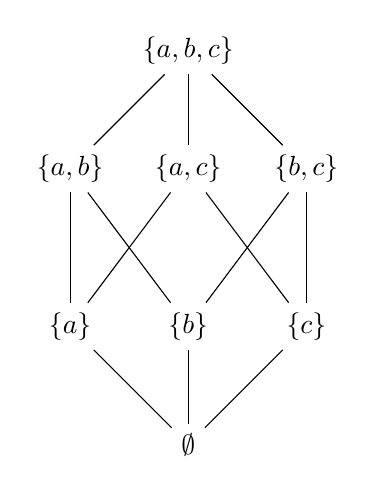
\begin{tikzpicture}
      \node (max) at (0, 5)		{$\{a, b, c\}$};
      \node (d1)   at (-1.5,3.5)	{$\{a, b\}$};
      \node (d2)   at (0,3.5)		 {$\{a, c\}$};
      \node (d3)   at (1.5,3.5)   {$\{b, c\}$};
      \node (a)   at (-1.5,1.5)	  {$\{a\}$};
      \node (b)   at (0,1.5)			{$\{b\}$};
      \node (c)   at (1.5,1.5)        {$\{c\}$};
      \node (min)   at (0, 0)  {$\emptyset$};
      
      \draw (min) -- (a);
      \draw (min) -- (b);
      \draw (min) -- (c);
      \draw (a) -- (d1);
      \draw (a) -- (d2);
      \draw (b) -- (d1);
      \draw (b) -- (d3);
      \draw (c) -- (d2);
      \draw (c) -- (d3);
      \draw (d1) -- (max);
      \draw (d2) -- (max);
      \draw (d3) -- (max);
      %\draw[preaction={draw=white, -,line width=6pt}] (a) -- (e) -- (c);
    \end{tikzpicture}
    \label{fig:DiagramaHasse3-A}
  }\quad\quad\quad %espaco separador
  \subfloat[Representação em forma de quase cubo.]{
    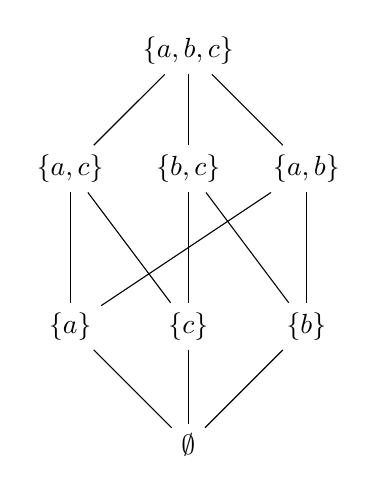
\begin{tikzpicture}
      \node (max) at (0, 5)		{$\{a, b, c\}$};
      \node (d1)   at (-1.5,3.5)	{$\{a, c\}$};
      \node (d2)   at (0,3.5)		 {$\{b, c\}$};
      \node (d3)   at (1.5,3.5)   {$\{a, b\}$};
      \node (a)   at (-1.5,1.5)	  {$\{a\}$};
      \node (b)   at (0,1.5)			{$\{c\}$};
      \node (c)   at (1.5,1.5)        {$\{b\}$};
      \node (min)   at (0, 0)  {$\emptyset$};
      
      \draw (min) -- (a);
      \draw (min) -- (b);
      \draw (min) -- (c);
      \draw (a) -- (d1);
      \draw (a) -- (d3);
      \draw (b) -- (d1);
      \draw (b) -- (d2);
      \draw (c) -- (d2);
      \draw (c) -- (d3);
      \draw (d1) -- (max);
      \draw (d2) -- (max);
      \draw (d3) -- (max);
      %\draw[preaction={draw=white, -,line width=6pt}] (a) -- (e) -- (c);
    \end{tikzpicture}
    \label{fig:DiagramaHasse3-B}
  }
  \caption{Diagramas de Hasse para o \textit{poset} $\langle \wp(\{a, b, c\}), \subseteq \rangle$.}
  \label{fig:DiagramaHasse3}
\end{figure}

\begin{exemplo}\label{exe:PosetCadeia}
	O \textit{poset} $\langle \{5, 6, 7, 8, 9\}, \leq \rangle$ é representado pelo diagrama a seguir.
\end{exemplo}
	
\begin{figure}[h]
  \centering
  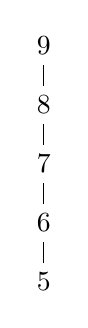
\begin{tikzpicture}
    \node (min) at (0, 0)  {$5$};
    \node (1)   at (0, 0.75)  {$6$};
    \node (2)   at (0, 1.5)  {$7$};
    \node (3)   at (0, 2.25)  {$8$};
    \node (4)   at (0, 3.0)  {$9$};
    
    \draw (min) -- (1) -- (2) -- (3) -- (4);
  \end{tikzpicture}
  \caption{Diagrama de Hasse do \textit{poset} $\langle \{5, 6, 7, 8, 9\}, \leq \rangle$}
  \label{fig:DiagramaHasse4}
\end{figure}

\textit{Posets} cuja ordem é total também são chamados de cadeias (ver \cite{abe1991-TC, morgado1962poset}) e nesse caso o diagrama será uma linha reta com todos os elementos sobre essa linha, exatamente como no Exemplo \ref{exe:PosetCadeia}. O leitor sem saber já usava esse conceito em seus estudo matemáticos a proferir frases como ``a reta real'' ou ``a reta dos números reais''. Agora obviamente dado um diagrama de Hasse sempre é possível recuperar a estrutura do \textit{poset} do mesmo, isto é, recuperar o conjunto base e a relação de ordem parcial que define o \textit{poset}, a seguir são apresentados alguns exemplos disto.

\begin{exemplo}
  Dado o diagrama de Hasse da Figura \ref{fig:DiagramaHasse5} a seguir,  dado que $6$ está ligado e abaixo de $3$ e $2$ tem-se que $(6,3), (6, 2) \in R$ onde $R$ é uma relação, o mesmo vale para os pares $(3, 5), (2, 4), (5, 1)$  e $(4, 1)$. Desse modo tal figura representa o \textit{poset} $\langle A, R \rangle$ em que $A = \{1, 2, 3, 4, 5, 6\}$ e $R$ corresponde a relação $\{(6,3), (6, 2), (3, 5), (2, 4), (5, 1), (4, 1), (6, 5), (6, 4), (6, 1), (2, 1), (5, 1)\} \cup Id_A$.
\end{exemplo}

\begin{figure}[h]
  \centering
  \begin{tikzpicture}
    \node (min)   at (0, 0)  {$6$};
    \node (1)   at (2, 2)  {$2$};
    \node (2)   at (-2, 2)  {$3$};
    \node (3)   at (2, 4)  {$4$};
    \node (4)   at (-2, 4)  {$5$};
    \node (max)   at (0, 6)  {$1$};
    
    \draw (min) -- (1) -- (3) -- (max);
    \draw (min) -- (2) -- (4) -- (max);
  \end{tikzpicture}
  \caption{Um diagrama de Hasse.}
  \label{fig:DiagramaHasse5}
\end{figure}


\begin{exemplo}
  Dado o diagrama de Hasse da Figura \ref{fig:DiagramaHasse6} representa o \textit{poset} $\langle B, R_B \rangle$ em que: $B = \{0, 1, 2, 3, 4, 5, 6\}$ e 
  $$R_B = Id_B \cup \{(5, 1), (6, 1), (1, 2), (2, 3), (2, 4)\} \cup  \{(5, 1), (6, 1), (1, 2), (2, 3), (2, 4)\}^+$$
\end{exemplo}

\begin{figure}[h]
  \centering
  \begin{tikzpicture}
    \node (min1)   at (2, 0)  {$6$};
    \node (min2)   at (-2, 0)  {$5$};
    \node (1)   at (0, 1)  {$1$};
    \node (2)   at (0, 3)  {$2$};
    \node (max1)   at (2, 4)  {$4$};
    \node (max2)   at (-2, 4)  {$3$};
    \node (min3) at (4, 0) {$0$};
    
    \draw (min1) -- (1) -- (2) -- (max1);
    \draw (min2) -- (1);
    \draw (2) -- (max2);
  \end{tikzpicture}
  \caption{Um diagrama de Hasse.}
  \label{fig:DiagramaHasse6}
\end{figure}

Como dito em \cite{carmo2013} um \textit{poset} é uma álgebra relacional ordenado, ou ainda, uma álgebra relacional, e como uma álgebra pode-se estudar: os elementos destacados, suas sub-álgebras (sub-estruturas) ou ainda os mecanismo de extensão da mesma. Na próxima seção este manuscrito irá realizar um estudo sobre os pontos.

\section{Elementos Notáveis de um \textit{Poset}}\label{sec:ElementosNotaveisPoset}

Como muito bem aprofundado em \cite{carmo2013, morgado1962poset, neggers1998poset}, existem diverso conceitos e aplicações interessantes ligados a ideia de \textit{posets}, assim para ajudar que leitor tenha uma formação sólida na área de teoria dos \textit{posets} é interessante apresentar alguns deste conceitos chaves da teoria, neste seção serão trabalhos os elementos notáveis existes nos \textit{posets} e suas propriedades.

\begin{definicao}[Máximo e Mínimo de um subconjunto]\label{def:MaxMinPoset}
	Seja $\langle A, \sqsubseteq \rangle$ um \textit{poset} e $X \subseteq A$ o máximo de $X$, denotado por $max(X)$, é um elemento $x \in X$ tal que para todo $y \in X$ tem-se que $y \sqsubseteq x$. O mínimo de $X$, denotado por $min(X)$,  é um elemento $x \in X$ tal que  para todo $y \in X$ tem-se que $x \sqsubseteq y$.
\end{definicao}

\begin{exemplo}
	Considere o \textit{poset} da Figura \ref{fig:DiagramaHasse1} para o conjunto $X = \{1, 2, a\}$ tem-se que $min(X) = 1$ e $max(X) = 2$.
\end{exemplo}

\begin{exemplo}
	Considere o \textit{poset} da Figura \ref{fig:DiagramaHasse2} para o conjunto $X = \{0, 1\}$ tem-se que $min(X) = 0$ e $max(X) = 1$.
\end{exemplo}

\begin{exemplo}
	Considere o \textit{poset} da Figura \ref{fig:DiagramaHasse3-A} para o conjunto $X = \{\{a, b\}, \{a\},$ $\{b\}, \emptyset\}$ tem-se que $min(X) = \emptyset$ e $max(X) = \{a, b\}$.
\end{exemplo}

Agora é conveniente ressaltar que tanto máximo quando o mínimo podem vir há não existir, isto é, dado um \textit{poset} $\langle A, \sqsubseteq \rangle$ um subconjunto $X$ de $A$ pode-se de tal forma que ele não contenha máximo e(ou) mínimo.

\begin{exemplo}
	Considere o \textit{poset} ilustrado pela Figura \ref{fig:DiagramaHasse5} o subconjunto $\{3, 2, 5, 4\}$ deste \textit{poset} não apresenta máximo e nem mínimo.
\end{exemplo}

\begin{exemplo}
	Considere o \textit{poset} ilustrado pela Figura \ref{fig:DiagramaHasse6} o subconjunto $\{1, 5, 6\}$ deste \textit{poset} possui máximo mas não possui mínimo.
\end{exemplo}

\begin{teorema}[Unicidade do máximo]\label{teo:UnicidadeMaximoPoset}
	Seja $\langle A, \sqsubseteq \rangle$ um \textit{poset} e $X \subseteq A$. Se existe $x \in X$ tal que $max(X) = x$, então $x$ é único.
\end{teorema}

\begin{prova}
	Dado $\langle A, \sqsubseteq \rangle$ um \textit{poset} e $X \subseteq A$. Suponha por absurdo que existem $x, x' \in X$ tal que $max(X) = x$ e $max(X) = x'$ com $x \neq x'$, logo por definição para todo $a \in X$ tem-se que $a \sqsubseteq x$ e $a \sqsubseteq x'$, mas desde que $x, x '\in X$ tem-se que $x \sqsubseteq x'$ e $x' \sqsubseteq x$ e, desde que, $\sqsubseteq$ é antissimétrica tem-se que $x = x'$ o que contradiz a hipótese e, portanto, se existe o máximo de $X$ ele é único.
\end{prova}

\begin{teorema}[Unicidade do mínimo]\label{teo:UnicidadeMinimoPoset}
	Seja $\langle A, \sqsubseteq \rangle$ um \textit{poset} e $X \subseteq A$. Se existe $x \in X$ tal que $min(X) = x$, então $x$ é único.
\end{teorema}

\begin{prova}
	Similar a demonstração do Teorema \ref{teo:UnicidadeMaximoPoset}.
\end{prova}

\begin{teorema}\label{teo:MonotonicidadeInclusaoMaxMin}
	Seja $\langle A, \sqsubseteq \rangle$ um \textit{poset} e $X, Y \subseteq A$ com $X \subseteq Y$ tem-se que:
	\begin{itemize}
		\item[(i)] Se $max(X) = a$ e $max(Y) = b$, então $a \sqsubseteq b$.
		\item[(ii)] Se $min(X) = a$ e $min(Y) = b$, então $b \sqsubseteq a$.
	\end{itemize}
\end{teorema}

\begin{prova}
	A demonstração é simples e fica como exercício ao leitor.
\end{prova}

Além da ideia de máximo e mínimo sobre os \textit{posets} também definido a ideia de maximais e minimais.

\begin{definicao}[Elementos maximais]\label{def:MaximaisPoset}
	Seja $\langle A, \sqsubseteq \rangle$ um \textit{poset}  um elemento $x \in A$ é dito ser um maximal se para todo $y \in A$ tem-se que se $x \sqsubseteq y$, então $x = y$.
\end{definicao}

\begin{exemplo}
  Considere o \textit{poset} esboçado pela Figura \ref{fig:DiagramaHasse7} a seguir. Para tal \textit{poset} tem-se que o elemento $g$ é um maximal e também é o máximo do conjunto.
\end{exemplo}

\begin{figure}[h]
  \centering
  \begin{tikzpicture}
    \node (a)   at (0, 0)  {$a$};
    \node (b) at (1, 1) {$b$};
    \node (c) at (2, 2) {$c$};
    \node (d) at (-2, 2) {$d$};
    \node (e) at (0, 2) {$e$};
    \node (f) at (1, 3) {$f$};
    \node (g) at (0, 4) {$g$};
    
    \draw (a) -- (b) -- (c);
    \draw (a) -- (d) -- (g);
    \draw (c) -- (f) -- (g);
    \draw (b) -- (e);
    \draw (e) -- (f);
  \end{tikzpicture}
  \caption{Um \textit{poset} representado por um diagrama de Hasse.}
  \label{fig:DiagramaHasse7}
\end{figure}

\begin{exemplo}
	Considere o \textit{poset} esboçado pela Figura \ref{fig:DiagramaHasse5}. Para tal \textit{poset} tem-se que o elemento $1$ é um maximal e também é o máximo do conjunto.
\end{exemplo}

Em algumas situações elementos maximais coincidem com o máximo, entretanto, como mostrado a seguir ser maximal não é garantia de ser o máximo do conjunto.

\begin{exemplo}
  Considere o \textit{poset} esboçado pela Figura \ref{fig:DiagramaHasse8} a seguir. Para tal \textit{poset} tem-se que os elementos $4$ e $5$ satisfazem a Definição \ref{def:MaximaisPoset} logo ambos são maximais do conjunto, porém, ambos são incomparáveis, portanto, nenhum é o máximo do conjunto.
\end{exemplo}

\begin{figure}[h]
  \centering
\begin{tikzpicture}
  \node (1)   at (0, 0)  {$1$};
  \node (2)   at (-1, 1)  {$2$};
  \node (3)   at (1, 1)  {$3$};
  \node (4)   at (0, 2)  {$4$};
  \node (5)   at (2, 2)  {$5$};
  
  \draw (1) -- (2) -- (4);
  \draw (1) -- (3) -- (4);
  \draw (3) -- (5);
\end{tikzpicture}
\caption{Um \textit{poset} representado por um diagrama de Hasse.}
\label{fig:DiagramaHasse8}
\end{figure}

De forma dual ao conceito de maximal pode-se definir a ideia de elemento minimal, e isto é feito como se segue.

\begin{definicao}[Elementos minimais]\label{def:MinimalPoset}
Seja $\langle A, \sqsubseteq \rangle$ um \textit{poset}  um elemento $x \in A$ é dito ser um minimal se para todo $y \in A$ tem-se que se $y\sqsubseteq x$, então $x = y$.
\end{definicao}

\begin{exemplo}
Considerando o \textit{poset} da Figura \ref{fig:DiagramaHasse7} tem-se que o elemento $a$ é minimal de tal conjunto e também apresenta a característica de ser o mínimo.
\end{exemplo}

\begin{exemplo}
Considerando o \textit{poset} da Figura \ref{fig:DiagramaHasse8} tem-se que o elemento $1$ é minimal de tal conjunto e também apresenta a característica de ser o mínimo.
\end{exemplo}

\begin{exemplo}
Considerando o \textit{poset} da Figura \ref{fig:DiagramaHasse6} tem-se que os elementos $5$ e $6$ são ambos minimais, porém, como são ambos incomparáveis tem-se que nenhum dos dois é o mínimo do conjunto base do \textit{poset}.
\end{exemplo}

\begin{exemplo}
Considere o \textit{poset} da Figura \ref{fig:DiagramaHasse9} a seguir, tem-se que $g$ e $f$ são elementos maximais e $c, a$ e $b$ são elementos minimais, note que tal \textit{poset} não possui máximo e mínimo.
\end{exemplo}

\begin{figure}[h]
\centering
\begin{tikzpicture}
  \node (a)   at (0, 0)  {$a$};
  \node (b)   at (2, 0)  {$b$};
  \node (c)   at (-2, 0)  {$c$};
  \node (d)   at (0, 1)  {$d$};
  \node (e)   at (0, 2)  {$e$};
  \node (f)   at (1, 3)  {$f$};
  \node (g)   at (-1, 3)  {$g$};
  
  \draw (d) -- (c);
  \draw (d) -- (a);
  \draw (d) -- (b);
  \draw (d) -- (e);
  \draw (e) -- (g);
  \draw (e) -- (f);
\end{tikzpicture}
\caption{Um \textit{poset} representado por um diagrama de Hasse.}
\label{fig:DiagramaHasse9}
\end{figure}

\begin{definicao}[Majorante]\label{def:Majorante}
	Seja $\langle A, \sqsubseteq \rangle$ um \textit{poset} e $X \subseteq A$, um elemento $x \in A$ é dito ser um majorante (ou cota superior) de $X$ sempre que para todo $y \in X$ tem-se que $y\sqsubseteq x$.
\end{definicao}

\begin{exemplo}
	Considere o \textit{poset} esboçado na Figura \ref{fig:DiagramaHasse9} e o subconjunto $X = \{e, d, c\}$ tem-se que os elementos $e, f$ e $g$ são todos majorantes de $X$. Já os subconjuntos $Y = \{g, f, e\}$ e $Z = \{g, f, a\}$ não possuem majorantes.
\end{exemplo}

\begin{exemplo}
	Considere o \textit{poset} esboçado na Figura \ref{fig:DiagramaHasse8} e o subconjunto $X = \{2, 3, 5\}$  não possui majorantes, já o conjunto $Y = \{1,2, 3, 4\}$ possui o elemento $4$ como majorante.
\end{exemplo}

\begin{exemplo}
	Considere o \textit{poset} esboçado na Figura \ref{fig:DiagramaHasse7} e o subconjunto $X = \{d, e, f\}$ tem-se que o elemento $g$ é o majorante de $X$.
\end{exemplo}

Como mencionado em \cite{abe1991-TC} se $x$ é um majorante (ou cota superior) de um conjunto $X$, é dito que $X$ é um conjunto majorado pelo elemento $x$ ou que o conjunto $X$ possui uma cota superior $x$.

\begin{definicao}[Conjunto dos majorantes]\label{def:ConjuntoDosMajorantes}
	Seja $\langle A, \sqsubseteq \rangle$ um \textit{poset} e $X \subseteq A$, o conjunto de todos os majorantes de $X$ é denotado por $X_\uparrow$.
\end{definicao}

Como dito em \cite{abe1991-TC, carmo2013, morgado1962poset} a maior parte dos conceito na teoria dos \textit{posets} tem natureza dual, assim é natural que seja imediatamente apresentadas as definições de minorantes e conjunto dos minorantes.

\begin{definicao}[Minorante]\label{def:Mjnorante}
	Seja $\langle A, \sqsubseteq \rangle$ um \textit{poset} e $X \subseteq A$, um elemento $x \in A$ é dito ser um minorante (ou cota inferior) de $X$ sempre que para todo $y \in X$ tem-se que $x\sqsubseteq y$.
\end{definicao}

\begin{exemplo}
	Considere o \textit{poset} esboçado na Figura \ref{fig:DiagramaHasse9} e o subconjunto $X = \{e, d, c\}$ tem-se que o elemento $c$ é o minorante de $X$. Já os subconjuntos $Y = \{g, f, e\}$ tem como minorantes os elementos $e, d, c, a$e $b$, por fim, para o conjunto $Z = \{g, f, a\}$ o único minorantes é o elemento $a$.
\end{exemplo}

\begin{exemplo}
	Considere o \textit{poset} esboçado na Figura \ref{fig:DiagramaHasse8} e o subconjunto $X = \{2, 3, 5\}$  tem como minorante o elemento $1$, já o conjunto $Y = \{3, 4, 5\}$ possui como minorantes os elementos $1$ e $3$.
\end{exemplo}

\begin{exemplo}
	Considere o \textit{poset} esboçado na Figura \ref{fig:DiagramaHasse7} e o subconjunto $X = \{d, e, f\}$ tem-se que o elemento $a$ é o único minorante deste conjunto, já para o conjunto $Y = \{g, f\}$ tem-se os elementos $f, e, c, b$ e $a$ como minorantes de $Y$.
\end{exemplo}

\begin{definicao}[Conjunto dos minorantes]\label{def:ConjuntoDosMjnorantes}
	Seja $\langle A, \sqsubseteq \rangle$ um \textit{poset} e $X \subseteq A$, o conjunto de todos os minorantes de $X$ é denotado por $X_\downarrow$.
\end{definicao}

\begin{teorema}
	Seja $\langle A, \sqsubseteq \rangle$ um \textit{poset} e $X \subset A$. Se $a \in A$ é um majorante (minorante) de $X$ e $a \in X$, então $a = max(X)$ $(a = min(X))$.
\end{teorema}

\begin{prova}
	Trivial.
\end{prova}

O próximo resultado estabelece que o conjunto de majorantes e minorantes respeita a monotonicidade da relação de inclusão.

\begin{teorema}\label{teo:MonotonicidadeMajoranteMinorante}
	Seja $\langle A, \sqsubseteq \rangle$ um \textit{poset} e $X, Y \subseteq A$. Se $X \subseteq Y$, então: 
	\begin{itemize}
		\item[(i)] $Y_\uparrow \subseteq X_\uparrow$.
		\item[(ii)] $Y_\downarrow \subseteq X_\downarrow$.
	\end{itemize}
\end{teorema}

\begin{prova}
	A demonstração é simples e ficará como exercício ao leitor. 
\end{prova}

\begin{definicao}[Conjunto limitado]\label{def:ConjuntoLimitadoPoset}
	Seja $\langle A, \sqsubseteq \rangle$ um \textit{poset} e $X \subseteq A$, o conjunto $X$ é dito ser limitado em $A$ sempre que $X$ possui majorantes e minorantes.
\end{definicao}

\begin{exemplo}
	Considere o \textit{poset} $\langle \mathbb{N}, \leq \rangle$ o conjunto $X_{k_1, k_2} = \{x \in \mathbb{N} \mid k_1 < x < k_2\}$ é um conjunto que sempre possuirá majorantes e minorantes (a saber $k_1$ e $k_2$) logo ele é um conjunto limitado em $\langle \mathbb{N}, \leq \rangle$.
\end{exemplo}

\begin{exemplo}
	Considere o \textit{poset} $\langle \wp(A), \subseteq \rangle$ onde $A$ é um conjunto qualquer, um conjunto $X \in \wp(A)$ sempre irá possuir minorante e majorante, que como dito em \cite{abe1991-TC} são gerados pela interseção e união respectivamente. Assim qualquer $X \in \wp(A)$ sempre será um conjunto limitado em $\langle \wp(A), \subseteq \rangle$.
\end{exemplo}

\begin{exemplo}
	Considere o \textit{poset} esboçado na Figura \ref{fig:DiagramaHasse9} e o subconjunto $X = \{e, d, c, a , b\}$ tem-se que tal conjunto possui os majorantes $e, g$ e $f$, mas não possui minorantes, assim $X$ não é limitado.
\end{exemplo}

\begin{teorema}\label{teo:MinoranteMajoranteInclusao}
	Seja $\langle A, \sqsubseteq \rangle$ um \textit{poset} e $X \subseteq A$. Se $X \neq \emptyset$, então $X \subseteq (X_\downarrow)_\uparrow$.
\end{teorema}

\begin{prova}
	Dado $\langle A, \sqsubseteq \rangle$ um \textit{poset} e $X \subseteq A$, suponha que $X \neq \emptyset$, assim para todo $x \in X$ e cada $y \in X_\downarrow$ tem-se que $y \sqsubseteq x$, logo $x \in (X_\downarrow)_\uparrow$, portanto, $X \subseteq (X_\downarrow)_\uparrow$.
\end{prova}

\begin{teorema}\label{teo:MajoranteMinoranteInclusao}
	Seja $\langle A, \sqsubseteq \rangle$ um \textit{poset} e $X \subseteq A$. Se $X \neq \emptyset$, então $X \subseteq (X_\uparrow)_\downarrow$.
\end{teorema}

\begin{prova}
	Similar a prova do Teorema \ref{teo:MinoranteMajoranteInclusao}.
\end{prova}

\begin{teorema}\label{teo:IdadeMajoranteMinorante}
	Seja $\langle A, \sqsubseteq \rangle$ um \textit{poset} e $X \subseteq A$. Se $X \neq \emptyset$, então:
	\begin{itemize}
		\item[(i)]  $X_\uparrow = ((X_\uparrow)_\downarrow)_\uparrow$.
		\item[(ii)] $X\downarrow = ((X_\downarrow)_\uparrow)_\downarrow$.
	\end{itemize}
\end{teorema}

\begin{prova}
	Dado $\langle A, \sqsubseteq \rangle$ um \textit{poset} e $X \subseteq A$. Suponha que $X \neq \emptyset$, assim tem-se que:
	\begin{itemize}
		\item[(i)] Pelo Teorema \ref{teo:MajoranteMinoranteInclusao} segue que $X_\uparrow \subseteq ((X_\downarrow)_\uparrow)_\downarrow$, por outro lado, pelo Teorema \ref{teo:MinoranteMajoranteInclusao} pode-se concluir que $((X_\uparrow)_\downarrow)_\uparrow \subseteq X_\uparrow$, portanto, pela Definição \ref{def:IgualdadeConjuntos} tem-se que  $X_\uparrow = ((X_\uparrow)_\downarrow)_\uparrow$.
		\item[(ii)] Similar ao item anterior.
	\end{itemize}
	Completando assim a prova.
\end{prova}

\begin{teorema}\label{teo:RotacaoMajoranteMinorante}
	Seja $\langle A, \sqsubseteq \rangle$ um \textit{poset} e $X, Y \subseteq A$. Se $X, Y \neq \emptyset$, então:
	\begin{itemize}
		\item[(i)]  $(X \cup Y)_\downarrow = X_\downarrow \cap Y_\downarrow$.
		\item[(ii)] $(X \cup Y)_\uparrow = X_\uparrow \cap Y_\uparrow$.
	\end{itemize}
\end{teorema}

\begin{prova}
	Dado $\langle A, \sqsubseteq \rangle$ um \textit{poset} e $X \subseteq A$. Suponha que $X \neq \emptyset$, assim tem-se que:
	\begin{itemize}
		\item[(i)] Desde que $X \subseteq X \cup Y$ e  $Y \subseteq X \cup Y$ tem-se pelo Teorema \ref{teo:MonotonicidadeMajoranteMinorante} que $(X \cup Y)_\downarrow \subseteq X_\downarrow$ e  $(X \cup Y)_\downarrow \subseteq Y_\downarrow $, consequentemente, $(X \cup Y)_\downarrow \subseteq X_\downarrow \cap Y_\downarrow$. Por outro lado, para todo $x \in X_\downarrow \cap Y_\downarrow$ tem-se para todo $y \in X$ que $x \leq y$ e para todo $z \in Y$ que $x \leq z$, assim $x \in (X \cup Y)_\downarrow$ e assim $(X \cup Y)_\downarrow \subseteq X_\downarrow \cap Y_\downarrow$ e, portanto, pela Definição \ref{def:IgualdadeConjuntos}  tem-se que $(X \cup Y)_\downarrow = X_\downarrow \cap Y_\downarrow$.
		\item[(ii)] Similar ao item anterior.
	\end{itemize}
	O que termina a prova.
\end{prova}

\begin{definicao}[Supremo]\label{def:Supermo}
	Seja $\langle A, \sqsubseteq \rangle$ um \textit{poset} e $X \subseteq A$ o supremo de $X$ (caso exista), denotado por $sup(X)$, é o menor dos majorantes, em notação formal tem-se que $sup(X) = min(X_\uparrow)$.
\end{definicao}

Como dito em \cite{abe1991-TC, carmo2013}, uma forma de caracterização do supremo é através de suas propriedades inerentes, e isto é feito da seguinte forma, dado um \textit{poset} $\langle A, \sqsubseteq \rangle$ tem-se que $sup(X) = a $ se, e somente se:

\begin{itemize}
	\item[1.] $a \in A$.
	\item[2.] Para todo $x \in X$ tem-se que $x \sqsubseteq a$.
	\item[3.] Se $a' \in A$ e para todo $x \in X$ tem-se que  $x \sqsubseteq a'$, então $a \sqsubseteq a'$.
\end{itemize}

Note que a propriedade (1) diz que o supremo (caso exista) é sempre um elemento do poset, já a propriedade (2) estabelece que o supremo deve ser um majorante e a propriedade (3) estabelece que o supremo deve ser a menor cota superior, isto é, o mínimo do conjunto dos majorantes.

\begin{definicao}[Ínfimo]\label{def:Infimo}
	Seja $\langle A, \sqsubseteq \rangle$ um \textit{poset} e $X \subseteq A$ o ínfimo de $X$ (caso exista), denotado por $inf(X)$, é o maior dos minorantes, em notação formal tem-se que $sup(X) = max(X_\downarrow)$.
\end{definicao}

Dualmente ao supremo como dito em \cite{abe1991-TC, carmo2013}, uma forma de caracterização do ínfimo é através de suas propriedades inerentes, e isto é feito da seguinte forma, dado um \textit{poset} $\langle A, \sqsubseteq \rangle$ tem-se que $inf(X) = a $ se, e somente se:

\begin{itemize}
	\item[1.] $a \in A$.
	\item[2.] Para todo $x \in X$ tem-se que $a \sqsubseteq x$.
	\item[3.] Se $a' \in A$ e para todo $x \in X$ tem-se que  $a' \sqsubseteq x$, então $a' \sqsubseteq a$.
\end{itemize}

Ou seja, a propriedade (1) diz que o ínfimo (caso exista) é sempre um elemento do poset, já a propriedade (2) estabelece que o  ínfimo deve ser um minorante e a propriedade (3) estabelece que o  ínfimo deve ser a maior cota inferior, isto é, o máximo do conjunto dos minorantes.

\begin{atencao}
  Com pode ser visto em \cite{carmo2013} e \cite{fmcbook}, os termos \textit{least upper bound} (menor cota superior) e \textit{join} são sinônimos de supremo, enquanto, que \textit{greatest lower bound} (maior cota inferior) e \textit{meet} são sinônimos de ínfimo.
\end{atencao}

\begin{exemplo}\label{exe:SupremoInfimoPoset}
	Considere o \textit{poset} representado pela Figura \ref{fig:DiagramaHasse10} a seguir, o subconjunto $X = \{2, 3, 4, 5\}$ é tal que $sup(X) = 7$ e $inf(X) = 2$, por lado, para o subconjunto $Y = \{1, 0, 2, 4\}$ tem-se que $sup(Y) = 3$ mas não existe um ínfimo de tal conjunto. Além disso, pegando o conjunto inteiro do \textit{poset} tem-se que o conjunto possui supremo, a saber $7$ mas não possui ínfimo. 
\end{exemplo}

\begin{figure}[h]
  \centering
  \begin{tikzpicture}
    \node (min1)   at (0, 0)  {$1$};
    \node (min2)   at (2, 0)  {$0$};
    \node (a) at (1, 1)  {$2$};
    \node (b)   at (0, 2)  {$4$};
    \node (c)   at (2, 2)  {$5$};
    \node (e) at (1, 3)  {$3$};
    \node (f) at (3, 3)  {$6$};
    \node (g) at (2, 4)  {$7$};
    
    \draw (min1) -- (a) -- (b) -- (e) -- (g);
    \draw (min2) -- (a) -- (c) -- (f) -- (g);
    \draw (c) -- (e);
  \end{tikzpicture}
  \caption{Diagrama de Hasse do \textit{poset} do Exemplo \ref{exe:SupremoInfimoPoset}.}
  \label{fig:DiagramaHasse10}
\end{figure}

\begin{exemplo}
  Considerando o \textit{poset} $\langle \mathbb{Q}, \leq \rangle$ tem-se que o subconjunto $\{x \in \mathbb{Q} \mid x^2 \leq 2\}$ não possui supremo pois $\sqrt{2} \notin \mathbb{Q}$.
\end{exemplo}

\begin{teorema}
	Seja $\langle A, \sqsubseteq \rangle$ um \textit{poset} e $X, Y \subseteq A$. Se $X \subseteq Y$ e além disso $X$ e $Y$ possuem supremo, então $sup(X) \sqsubseteq sup(Y)$.
\end{teorema}

\begin{prova}
	Dado $\langle A, \sqsubseteq \rangle$ um \textit{poset} e $X, Y \subseteq A$, assuma $X \subseteq Y$ e que que $X$ e $Y$ possuem supremo, assim pelo Teorema \ref{teo:MonotonicidadeMajoranteMinorante}(i) tem-se que $Y_\uparrow \subseteq X_\uparrow$.  Mas pelo Teorema \ref{teo:MonotonicidadeInclusaoMaxMin}(ii) tem-se que $min(Y_\uparrow) \sqsubseteq min(X_\uparrow)$, logo $sup(X) \sqsubseteq sup(Y)$.
\end{prova}

\begin{teorema}
	Seja $\langle A, \sqsubseteq \rangle$ um \textit{poset} e $X, Y \subseteq A$. Se $X \subseteq Y$ e além disso $X$ e $Y$ possuem ínfimo, então $inf(Y) \sqsubseteq inf(X)$.
\end{teorema}

\begin{prova}
	Dado $\langle A, \sqsubseteq \rangle$ um \textit{poset} e $X, Y \subseteq A$, assuma $X \subseteq Y$ e que que $X$ e $Y$ possuem supremo, assim pelo Teorema \ref{teo:MonotonicidadeMajoranteMinorante}(ii) tem-se que $Y_\uparrow \subseteq X_\uparrow$.  Mas pelo Teorema \ref{teo:MonotonicidadeInclusaoMaxMin}(i) tem-se que $max(Y_\downarrow) \sqsubseteq max(X_\downarrow)$, logo $inf(Y) \sqsubseteq inf(X)$.
\end{prova}

\begin{teorema}\label{teo:InfimoApartirSupremo}
	Se $\langle A, \sqsubseteq \rangle$ é um \textit{poset}, $X \subseteq A$ com $sup(X_\downarrow) = a$ e $a \in A$, então $inf(X) = sup(X_\downarrow) $.
\end{teorema}

\begin{prova}
	$\langle A, \sqsubseteq \rangle$ é um \textit{poset}, $X \subseteq A$ com $sup(X_\downarrow) = a$ e $a \in A$, agora note que para qualquer que seja $x \in X$ e $y \in X_\downarrow$ tem-se que $y \sqsubseteq x$, e assim $x$ é claramente um majorante de $X_\downarrow$, ou seja, $x \in (X_\downarrow)_\uparrow$,  consequentemente, $a \sqsubseteq y$, uma vez que, $sup(X_\downarrow) = a$, assim $a$ é um minorante de $X$, ou seja, $a \in X_\downarrow$. Por outro lado, para qualquer $z \in X_\downarrow$ tem-se que $z \sqsubseteq a$ e, portanto, $a = inf(X)$.
\end{prova}

\begin{teorema}\label{teo:SupremoApartirInfimo}
	Se $\langle A, \sqsubseteq \rangle$ é um \textit{poset}, $X \subseteq A$ com $inf(X_\downarrow) = a$ e $a \in A$, então $sup(X) = inf(X_\uparrow) $.
\end{teorema}

\begin{prova}
	Similar a demonstração do Teorema \ref{teo:InfimoApartirSupremo}.
\end{prova}

Quando um conjunto $X$ satisfaz o Teorema  \ref{teo:InfimoApartirSupremo} é dito que ele é inferiormente limitado, e quando ele satisfaz o Teorema \ref{teo:SupremoApartirInfimo} é dito que ele é superiormente limitado. Quando ele satisfaz os dois então ele satisfaz a Definição \ref{def:ConjuntoLimitadoPoset}.

\begin{teorema}
	Se $\langle A, \sqsubseteq \rangle$ é um \textit{poset}, então as seguintes asserções são equivalentes:
	\begin{itemize}
		\item[(1)] Todo subconjunto não vazio superiormente limitado de $A$ possui supremo.
		\item[(2)] Todo subconjunto não vazio inferiormente limitado de $A$ possui ínfimo.
	\end{itemize}
\end{teorema}
	
\begin{prova}
	Dado $\langle A, \sqsubseteq \rangle$ um \textit{poset}, tem-se que:
	
	$(1) \Rightarrow (2)$ Assuma que todo subconjunto não vazio superiormente limitado de $A$ possui supremo, agora seja $X \subseteq A$ limitado inferiormente, ou seja, $X_\downarrow \neq \emptyset$, agora obviamente cada $x \in X$ é tal que $x$ é um majorante de $X_\downarrow$, ou seja, $x \in (X_\downarrow)_\uparrow$ e, portanto, $X_\downarrow$ é superiormente limitado, logo pelo Teorema \ref{teo:SupremoApartirInfimo} existe o supremo do conjunto $X_\downarrow$, consequentemente pelo Teorema \ref{teo:InfimoApartirSupremo} existe o ínfimo de $X_\downarrow$.
	
	$(2) \Rightarrow (1)$ Similar ao item anterior.
\end{prova}

\section{Boa Ordenação e Relações Bem Fundadas}\label{sec:BoaOrdem}

Agora que o leitor chegou até este ponto significa que está pronto para a apresentação ligada a ideia de boas ordens e ordem bem fundadas.

\begin{definicao}[Boa ordem]\label{def:BoaOrdem}
	Uma ordem parcial $\sqsubseteq$ sobre um conjunto $A$ é dita uma boa ordem sempre que para todo subconjunto não vazio $B$ de $A$ é tal que $B$ possui elemento mínimo com respeito a ordem $\sqsubseteq$.
\end{definicao}

O leitor mais atento pode ter notado que Definição \ref{def:BoaOrdem} oculta o fato de que uma boa ordem é necessariamente um ordem total. Como dito em \cite{joaoPavao2014}, sempre que $\sqsubseteq$ for uma boa ordem a estrutura $\langle A, \sqsubseteq \rangle$ será chamada de conjunto bem ordenado.

\begin{exemplo}\label{exe:BoaOrdem}
	A relação $\leq$ é uma boa ordem com respeito ao conjunto dos números naturais, entretanto, se considerada sobre o conjuntos dos números inteiros ou reais ele não se classifica mais como uma boa ordem. 
\end{exemplo}

\begin{teorema}\label{teo:BoaOrdem}
	Uma estrutura $\langle A, \sqsubseteq \rangle$  é um conjunto bem ordenado se, e somente se, todo subconjunto não vazio de $A$ possui elemento mínimo.
\end{teorema}

\begin{prova}
	$(\Rightarrow)$ A ida é trivial pela própria Definição \ref{def:BoaOrdem}. $(\Leftarrow)$ Assuma que todo subconjunto não vazio de $A$ possui elemento mínimo, assim existe $z = min(A)$ e além disso tem-se que, dado $x, y \in A$ tem-se que $\{x, y\}$ tem menor elemento, ou seja, uma das três possibilidades acontece, $x \sqsubset y, y \sqsubset x$ ou $y = x$, entretanto, isso implica que qualquer dois elementos de $A$ são comparáveis e, portanto, $\sqsubseteq$ é um ordem total é assim $\langle A, \sqsubseteq \rangle$ é um conjunto bem ordenado.
\end{prova}

Note que a volta na demonstração do Teorema \ref{teo:BoaOrdem} estabelece que uma ordem ser total é uma condição necessária para que ela seja uma boa ordem, por outro lado, o exemplo \ref{exe:BoaOrdem} mostra que nem toda ordem total é de fato uma boa ordem. A seguir é apresentado o princípio da boa ordenação, neste texto não será apresentado sua demonstração, entretanto, é interessante que o leitor saiba que tal princípio foi apresentado pelo grande matemático Ernst Zermelo\sidefootnote{Zermelo junto com Adolf Abraham Halevi Fraenkel (1891-1965) desenvolveu o sistema formal hoje conhecido como teoria axiomática dos conjuntos.} (1871-1953), e que tal princípio é equivalente ao axioma da escolha \cite{carmo2013} (tratado em momentos futuros deste manuscrito).

\begin{principio}[Princípio da Boa Ordenação]\label{pri:BoaOrdenacao}
	Sobre qualquer conjunto $A$ é possível definir uma boa ordem $\unlhd$. 
\end{principio}

Pode-se agora apresentar um enfraquecimento da noção de boa ordem, que terá grande importância quando este manuscrito estiver tratado dos conceitos de indução, estruturas indutivamente geradas e recursão.

\begin{definicao}[Relação Bem Fundada]\label{def:RelacaoBemFundada}
	Uma relação binária $R$ sobre um conjunto $A$ é dita ser bem fundada, se não existem cadeias descendentes infinitas, em outras palavras, não existem elementos $a_0, a_1, a_2, \cdots \in A$ tal que, $\cdots \unlhd a_n \unlhd a_{n-1} \unlhd \cdots \unlhd a_2 \unlhd a_1 \unlhd a_0$.  
\end{definicao}

Observe que Definição \ref{def:RelacaoBemFundada} estabelece que a cadeia relacional não pode crescer infinitamente na direção da esquerda da relação, e portanto, deve existir um elemento no conjunto que seria visto com ponto extremo esquerdo da relação. Além disso, ainda pela a Definição \ref{def:RelacaoBemFundada} é notável que uma relação bem fundada pode ser não é transitiva, considere por exemplo a relação sobre os naturais da forma $R = \{(x, y) \in \mathbb{N}^2 \mid y = x + 1\}$, ela atende claramente as condições para ser uma relação bem fundada, entretanto, perceba que ela não é transitiva pois obviamente $0 \mathrel{R}1, 1 \mathrel{R} 2$ mas $0 \centernot{R} 2$, portanto, ela é bem fundada mas não é transitiva.

\begin{exemplo}\label{exe:RelacaoBemFundada1}
	Dado o conjunto dos números naturais as relações $<$ e $\leq$ são respectivamente uma relação bem fundada e um uma relação que não é bem fundada.
\end{exemplo}

\begin{exemplo}\label{exe:RelacaoBemFundada2}
	Dado o conjunto dos números inteiros tem-se que a relação $<$ não é bem fundada.
\end{exemplo}

\begin{exemplo}\label{exe:RelacaoBemFundada3}
	Dado o conjunto $A = \{0, 1, 2, 3, 4, 5, 6, 7, 8, 9\}$ a relação $\subset$ é uma relação bem fundada sobre $\wp(A)$.
\end{exemplo}

A seguir serão apresentados alguns resultados interessantes sobre as relação bem fundadas, em especial será apresentado uma forma de caracterização das relações bem fundadas.

\begin{proposicao}\label{prop:IrreflexividadeDaRelacaoBemFundada}
	Se $R$ é uma relação bem fundada em $A$, então $R$ é irreflexiva.
\end{proposicao}

\begin{prova}
	Suponha por absurdo que $R$ é uma relação bem fundada sobre um conjunto $A$ e que $R$ é reflexiva, logo para todo $a \in A$ tem-se que $a \mathrel{R} a$ e, portanto, existe uma cadeia infinita da seguinte forma $\cdots \mathrel{R} a \mathrel{R} a\mathrel{R} \cdots \mathrel{R} a \mathrel{R} a \mathrel{R} a$ o que contradiz a hipótese de $R$ seja uma relação bem fundada. Consequentemente, se $R$ é uma relação bem fundada, então ela deve ser irreflexiva.
\end{prova}

\begin{teorema}[Teorema de Caracterização]\label{teo:CaracterizacaoRelacaoBemFundada}
	Seja $\unlhd$ uma relação binária sobre $A$. Tem-se que $\unlhd$ é uma relação bem fundada se, e somente se, todo subconjunto não vazio $X$ de $A$ possui elemento minimal\footnote{O sentido de minimal aqui extrapola a ideia de minimal em respeito a ordem, visto que $\unlhd$ não é necessariamente um ordem parcial, aqui o sentido de minimal é que: $x \in X$ e não existe um $a \in X$ com $a \unlhd x$}.
\end{teorema}

\begin{prova}
	$(\Rightarrow)$ Suponha por absurdo que $\unlhd$ é uma relação bem fundada  e que existe um subconjunto não vazio $X$ de $A$ que não possui elemento minimal, assim sendo $X = \{a_1, a_2, \cdots\}$ tem-se que $a_1$ em $X$ não é minimal, logo existe $a_2$ em $X$ tal que $a_2 \unlhd a_1$, mas como $a_2$ também não é minimal existe um $a_3$ tal que $a_3 \unlhd a_2$ e assim sucessivamente, consequentemente, existindo uma cadeia infinita a esquerda da forma, $\cdots \unlhd a_3 \unlhd a_2 \unlhd a_1$, mas isso contradiz a hipótese de $\unlhd$ se uma relação bem fundada e, portanto, tem-se que se $\unlhd$ é bem fundada, todo subconjunto não vazio $X$ de $A$ irá possuir (pelo menos um) elemento minimal. $(\Leftarrow)$ Suponha por absurdo que $\unlhd$ não é uma relação bem fundada e que todo subconjunto não vazio $X$ de $A$ possui elemento minimal (logo existe $x \in X$ e não existe um $a \in X$ com $a \unlhd x$). Como $\unlhd$ não é bem fundada pode-se assumir que exista uma cadeia infinita a esquerda $\cdots \unlhd a_3 \unlhd a_2 \unlhd a_1$, agora deixe $a_i$ ser o elemento minimal de $X$ logo não pode existir um $a_{i+1}$ tal que $a_{i+1} \unlhd a_i$ o que contradiz a hipótese da existência da cadeia infinita, ou seja, contradiz a hipótese de $\unlhd$ não ser bem fundada, consequentemente, pode-se afirma que, se  todo subconjunto não vazio $X$ de $A$ possui elemento minimal, então $\unlhd$ é uma relação bem fundada.
\end{prova}

O próximo resultado revela ao leitor o estreito relacionamento entre a boa ordem e as relações bem fundadas, o resultado mostra que ser boa ordem é condição suficiente para ser uma relação bem fundado, porém ser bem fundada não é suficiente para ser uma boa ordem, ou seja, em um certo sentido as relação bem fundadas são mais exigentes.

\begin{teorema}\label{teo:RelacoesBemFundada-BoaOrdem}
	Seja $\langle A, \unlhd \rangle$ uma álgebra relacional tem-se que:
	\begin{itemize}
		\item[(i)] Se $\unlhd$ é uma boa ordem, então $\unlhd$ é uma relação bem fundada.
		\item[(ii)] Se $\unlhd$ é uma relação bem fundada e total\footnote{A totalidade de uma relação bem fundada $\unlhd$ está associado a ideia que quais $x, y \in A$ são comparáveis por $\unlhd$.}, então $\unlhd$ é uma boa ordem.
	\end{itemize}
\end{teorema}

\begin{prova}
	Dado uma álgebra relacional $\langle A, \unlhd \rangle$ tem-se que:
	\begin{itemize}
		\item[(i)] Suponha que $\unlhd$ é uma boa ordem, assim pela Definição \ref{def:BoaOrdem} tem-se que todo subconjunto não vazio de $A$ tem elemento mínimo, como todo elemento mínimo é também um minimal tem-se pelo Teorema \ref{teo:CaracterizacaoRelacaoBemFundada} que $\unlhd$ é uma relação bem fundada.
		\item[(ii)] Assuma que $\unlhd$ é uma relação bem fundada e total, logo tem-se que:
		\begin{itemize}
			\item Por $\unlhd$ ser bem fundada pela Proposição \ref{prop:IrreflexividadeDaRelacaoBemFundada} tem-se que $R$ é irreflexiva.
			\item Agora pela totalidade de $\unlhd$ tem-se para quaisquer $x, y, z \in A$ tais que $x \unlhd y$ e $y \unlhd z$ tem-se que $x = z$ iria implicar em uma cadeia infinita à esquerda, o que é impossível uma vez que $\unlhd$ é uma relação bem fundada, por outro lado, se $z \unlhd x$ fosse possível novamente seria possível construir uma cadeia infinita à esquerda o que novamente é um absurdo pelo fato de $\unlhd$ ser bem fundada, logo tem-se que $x \unlhd z$ e, portanto, $\unlhd$ é transitiva.
		\end{itemize}
	\end{itemize}
	Pelo fato de $\unlhd$ ser transitiva, irreflexiva e total tem-se que $R$ será uma ordem total estrita. Agora pelo Teorema \ref{teo:CaracterizacaoRelacaoBemFundada} uma vez que $\unlhd$ é bem fundada tem-se que todo subconjunto não vazio $X$ de $A$ possui elemento minimal $x$, entretanto, em um ordem total todo minimal é mínimo (provar isto fica como exercício), consequentemente, pela Definição \ref{def:BoaOrdem} tem-se que $\unlhd$ é uma boa ordem.
\end{prova}

\section{Operações Entre \textit{Posets}, Novas Ordens e Ordem Lexicográfica}\label{sec:OperacoesPoset}

Como dito em \cite{morgado1962poset}, diversas operações podem ser definidas entre \textit{posets}, além disso, é muito comum dado dois \textit{posets} $\langle A, \sqsubseteq_A \rangle$ e $\langle B, \sqsubseteq_B \rangle$ buscar definir novas ordens parciais sobre os conjuntos $A \cup B$ e $A \times B$ usando como base as ordens pré-existentes $\sqsubseteq_A$ e $\sqsubseteq_B$. Nesta seção serão estudadas operações entre \textit{posets} e também e como construir novas ordens parciais a partir de ordens parciais já existentes.

\begin{definicao}[Soma Cardinal]\label{def:SomaCardinal}
	Dado dois \textit{posets} $\langle A, \sqsubseteq_A \rangle$ e $\langle B, \sqsubseteq_B \rangle$ tal que $A \cap B = \emptyset$, a soma cardinal destes dois \textit{posets}, denotado por $A \boxplus B$, consiste no \textit{poset} $\langle A \cup B, \sqsubseteq_\boxplus \rangle$, onde $x \sqsubseteq_\boxplus y$ se, e somente se, $x \sqsubseteq_A y$ ou $x \sqsubseteq_B y$.
\end{definicao}

Apesar de não estar explicitamente escrito, note que, a Definição  \ref{def:SomaCardinal} estabelece que $x \sqsubseteq_\boxplus y$ acontece em apenas dois casos específicos, no primeiro caso ($x \sqsubseteq_A y$) tem -se $x, y \in A$, já no segundo caso ($x \sqsubseteq_B y$) obrigatoriamente $x, y \in B$, em qualquer outra situação os elementos $x$ e $y$ pertenceram a conjuntos distintos e nesse cenário eles serão incomparáveis, assim a relação $\sqsubseteq_\boxplus$ beira a trivialidade. Claramente o diagrama de Hasse para a ordem $\sqsubseteq_\boxplus$ é basicamente um diagrama em que os diagramas das ordens $\sqsubseteq_A$ e $\sqsubseteq_B$ são posto lado a lado, o exemplo a seguir ilustra esta ideia.

\begin{exemplo}
  Considerando os conjuntos $A = \{1, 4, 7\}$ e $B = \{a, b, c, d\}$ ordenados respectivamente pelas ordens $R_1$ e $R_2$ descritas pelos diagramas \ref{fig:DiagramaBase-A} e \ref{fig:DiagramaBase-B} da Figura \ref{fig:PosetsParaSomaCardinal1}, e a soma cardinal de ambos os \textit{posets} é representada pelo diagrama (destacado com linhas vermelhas) \ref{fig:SomaCardinal1} da Figura \ref{fig:PosetsParaSomaCardinal1}.
\end{exemplo}

\begin{figure}[h]
  \centering
  \subfloat[Poset $\langle A, R_1\rangle$.]{
    \begin{tikzpicture}
      \node (n1)  at  (2, 0){ };
      \node (n2)  at  (-2, 0){ };
      \node (m1)  at  (0, 0){$4$};
      \node (m2)  at  (0, 1.5){$1$};
      \node (m3)  at  (0, 3){$7$};
      
      \draw (m3) -- (m2) -- (m1);
      %\draw[preaction={draw=white, -,line width=6pt}] (a) -- (e) -- (c);
    \end{tikzpicture}
    \label{fig:DiagramaBase-A}
  }%\hfill %espaco separador
  \subfloat[Poset $\langle B, R_2\rangle$.]{
    \begin{tikzpicture}
      \node (m1)  at  (0, 0){$a$};
      \node (m2)  at  (2, 1.5){$b$};
      \node (m3)  at  (-2, 1.5){$c$};
      \node (m4)  at  (0, 3){$d$};
      
      
      \draw (m1) -- (m2) -- (m4);
      \draw (m1) -- (m3) -- (m4);
      %\draw[preaction={draw=white, -,line width=6pt}] (a) -- (e) -- (c);
    \end{tikzpicture}
    \label{fig:DiagramaBase-B}
  }\quad\quad\quad  
  \subfloat[Soma cardinal $A \boxplus B$]{
    \begin{tikzpicture}
      \node (n1)  at  (4.5, 0){$4$};
      \node (n2)  at  (4.5, 1.5){$1$};
      \node (n3)  at  (4.5, 3){$7$};
      
      \node (m1)  at  (2, 0){$a$};
      \node (m2)  at  (4, 1.5){$b$};
      \node (m3)  at  (0, 1.5){$c$};
      \node (m4)  at  (2, 3){$d$};
      
      \draw[color=red] (n1) -- (n2) -- (n3);
      \draw[color=red] (m1) -- (m2) -- (m4);
      \draw[color=red] (m1) -- (m3) -- (m4);
      %\draw[preaction={draw=white, -,line width=6pt}] (a) -- (e) -- (c);
    \end{tikzpicture}
    \label{fig:SomaCardinal1}
  }
  \caption{Dois \textit{Posets} e sua soma cardinal.}
  \label{fig:PosetsParaSomaCardinal1}
\end{figure}

{\color{red} Terminar de escrever a seção de operações sobre \textit{Poset} depois!!!!}

\section{Questionário}\label{sec:Questionario4part1}

{\color{red} Escrever depois. . .}
